The first test is devoted to investigating the distribution of the velocities of the particles after sufficiently long time. From statistical mechanics, we know that the velocities of a $2$-dimensional gas at equilibrium will distribute according to Maxwell's velocity distribution: 
\[
	p(v) = \frac{mv}{k_B T} \exp{\left(- \frac{mv^2}{2 k_B T}\right)},
\]
where $k_B$ is Boltzmann's constant, $T$ the absolute temperature, and $m$ the mass of the particles. It is essential that the all the particles have the same mass $m$, as will become apparent in section \ref{sec:mix1} and \ref{sec:mix2}.

We initialise an system of particles with velocities $\mathbf{v} = [v_0 \cos{\theta} , v_0 \sin{\theta}]$ with $\theta \sim \U[0,2\pi]$. The initial distribution of the velocities is therefore $C\delta (v - v_0)$. After simulating the system until equilibrium is reached, i.e. the the average number of particle collision is $\gg 1$, the distribution is as shown in figure \ref{fig:dist_1}. For this simulation, the stop criterion used was that the average number of collisions surpassed $50$. Judging from the plot, it seems to be sufficient for equilibrium to be reached. 

\begin{figure}[htb]
	\centering
	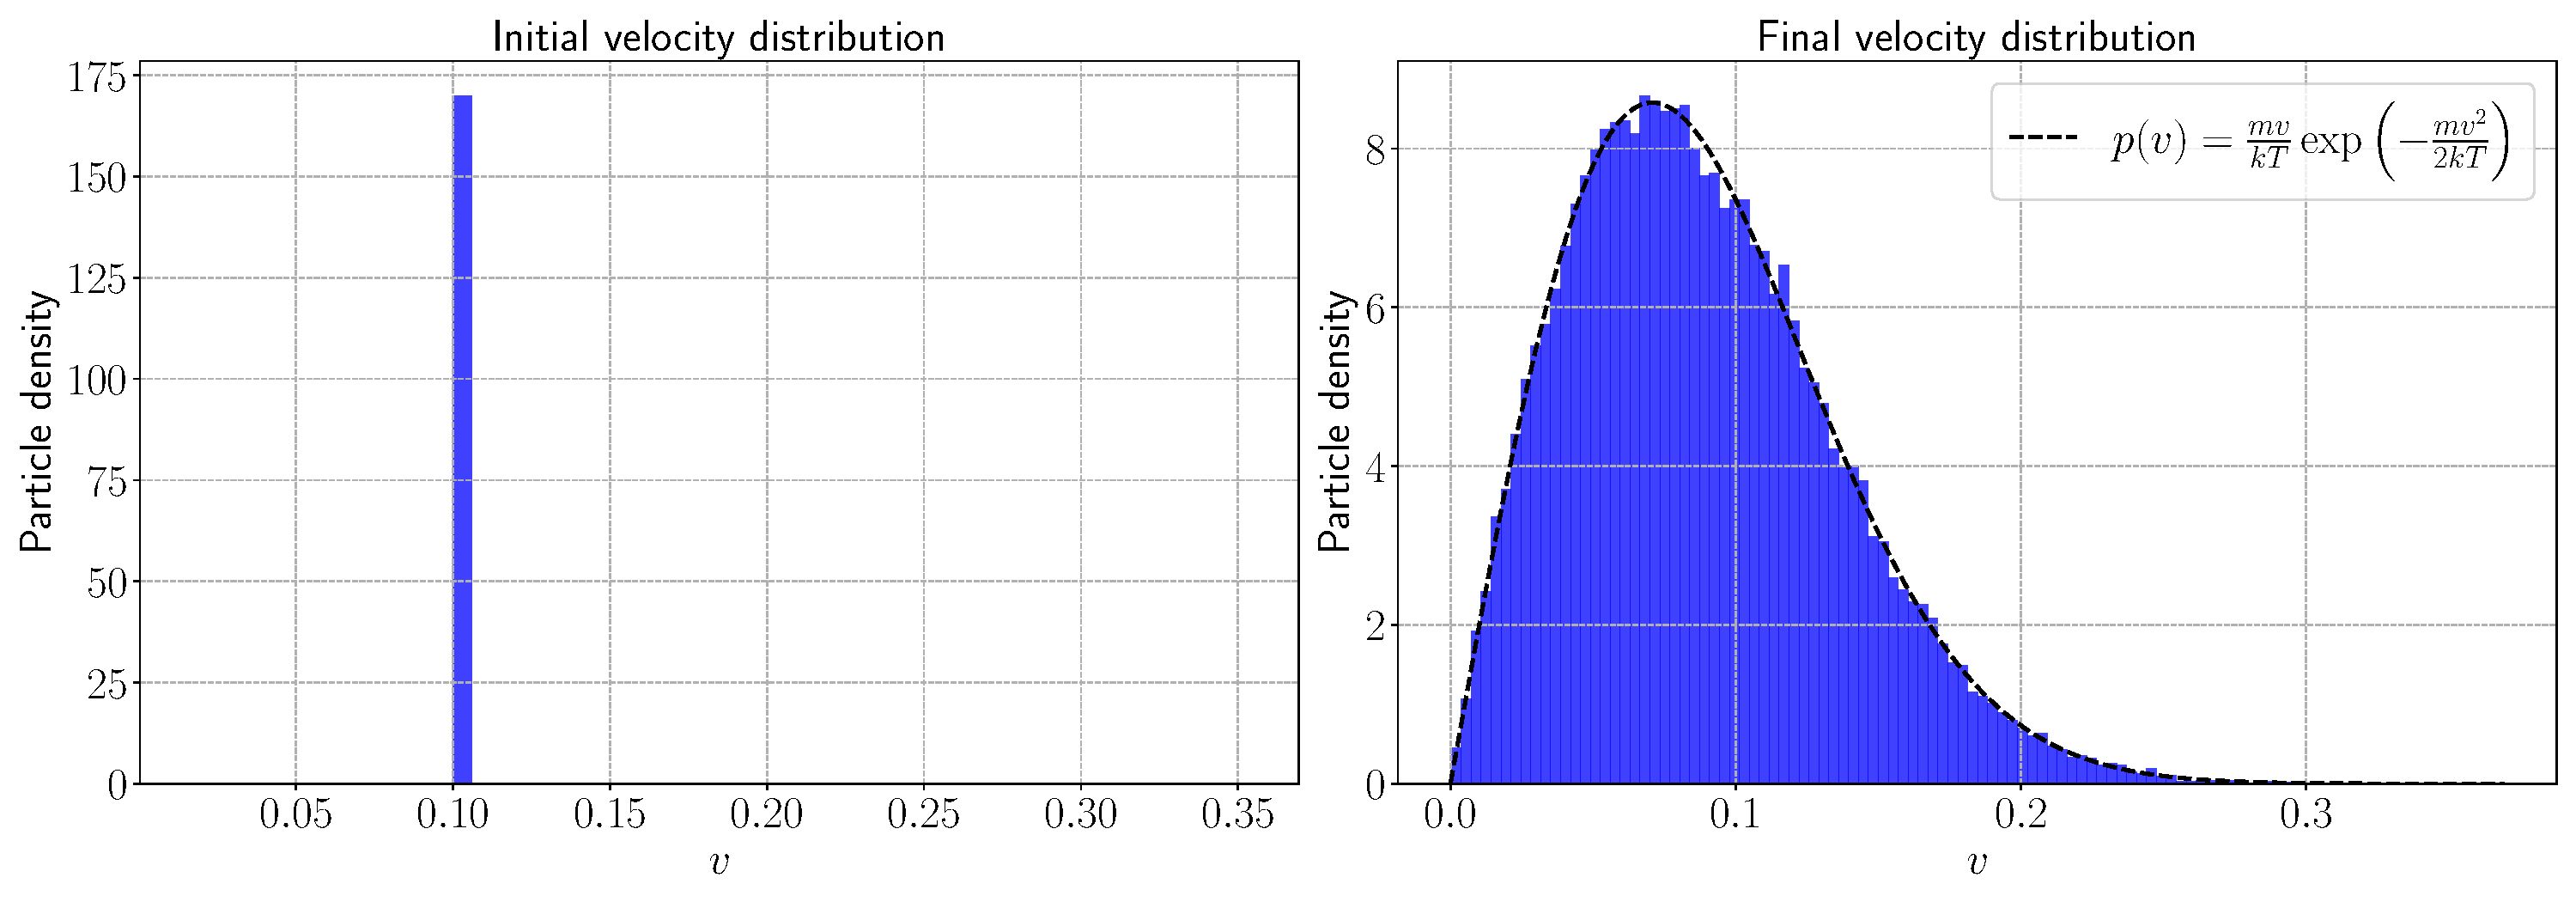
\includegraphics[width=\textwidth]{../fig/distribution}
	\caption{Distribution of velocities in a gas of $50000$ particles.}
	\label{fig:dist_1}
\end{figure}

To make the comparison more quantitative, we plot the difference between the Gaussian kernel density estimation of the final distribution and the Maxwell distribution. 

\begin{figure}[htb]
	\centering
	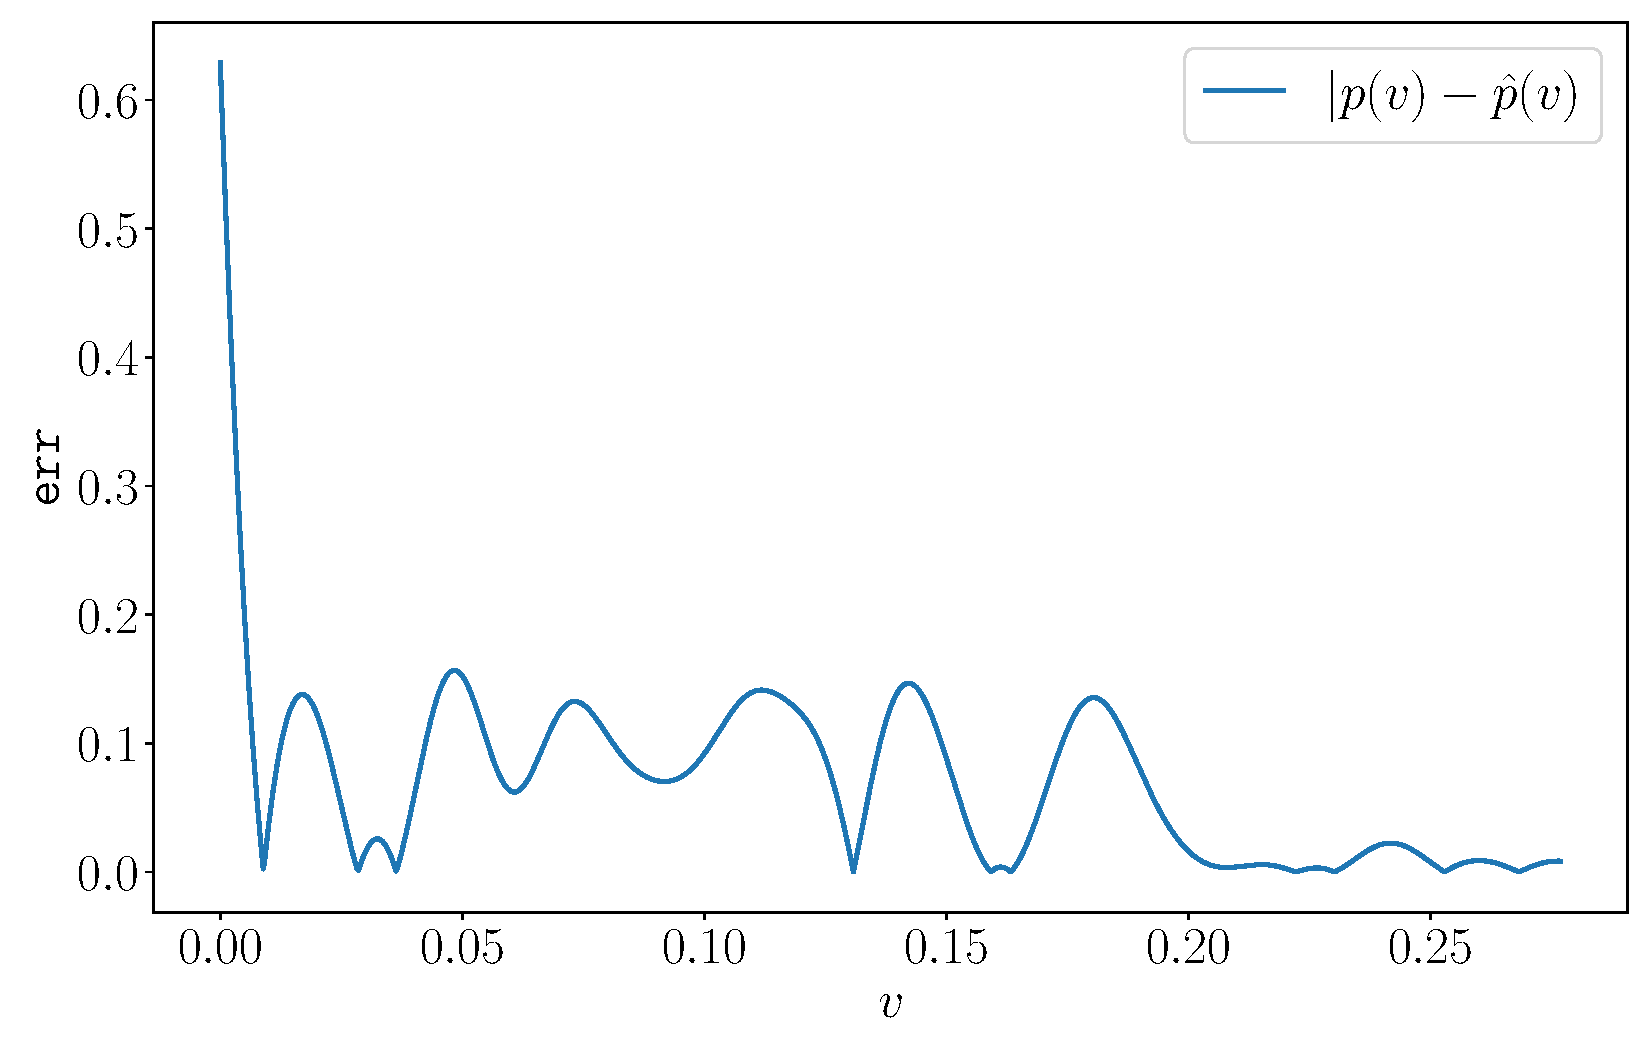
\includegraphics[width=0.8\textwidth]{../fig/kde_diff}
	\caption{Deviation between Gaussian kernel density estimation of the velocity distribution, $\hat{p}(v)$ and the Maxwell-distribution $p(v)$.}
	\label{fig:dist_2}
\end{figure}